\begin{figure*}[t]
  \centering
  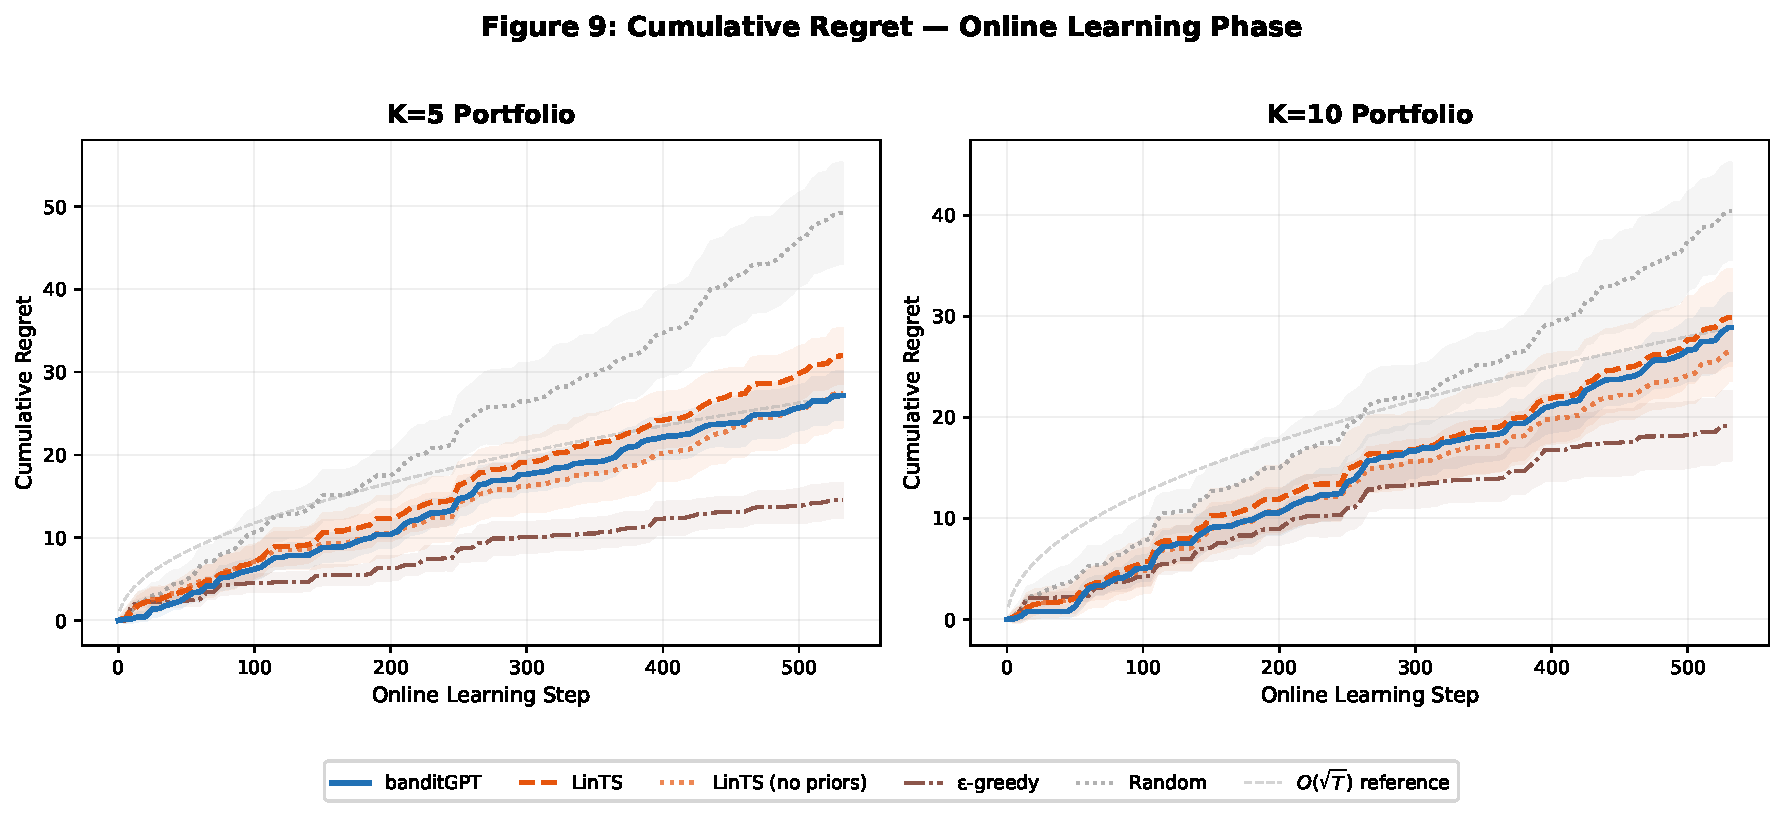
\includegraphics[width=\textwidth]{experiments/08_figure/results/figure9_cumulative_regret.pdf}
  \caption{
    \textbf{Cumulative Regret During Online Learning ($K{=}5$, $K{=}10$).}
    Regret at step $t$ is defined as $r_t = \max_{a \in \mathcal{A}} \mu_a(x_t) - \mu_{a_t}(x_t)$,
    i.e., the gap between the per-prompt oracle reward and the reward of the
    selected model.
    \emph{Left:} $K{=}5$ portfolio; \emph{Right:} $K{=}10$ portfolio.
    banditGPT achieves the lowest cumulative regret among contextual bandits
    at $K{=}5$ (27.1 vs.\ 31.9 for LinTS, $-15\%$) and is competitive at $K{=}10$
    (28.9 vs.\ 29.9).
    Both contextual methods track below the $O(\sqrt{T})$ reference curve
    (grey dashed), confirming sub-linear regret growth consistent with
    theoretical guarantees for linear bandits.
    The $\varepsilon$-greedy baseline achieves the lowest training regret
    by greedily exploiting the single best-on-average model, but---unlike
    the contextual methods---cannot adapt its routing per prompt
    (see Section~\ref{sec:multimodel} for holdout evaluation).
    Shaded bands denote $\pm 1\sigma$ across 20 trials.
  }
  \label{fig:cumulative_regret}
\end{figure*}
